\subsection{Feature importances}

\begin{figure}
\centering
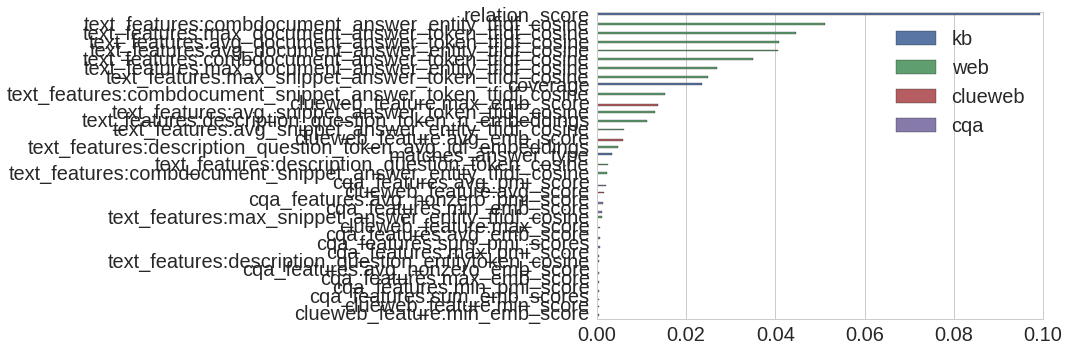
\includegraphics[width=0.5\textwidth]{img/feature_importances}
\caption{Importances of different text-based features for KBQA}
\label{fig:feature_importances}
\end{figure}

Figure \ref{fig:feature_importances} plots importances of different text-based features we use in Text2KB.
As we can see, web-search results based features ranked higher than CQA and ClueWeb-based features.

\subsection{Wins and Loses}

Show examples of questions, which are fixed by different components of the proposed system.

We can also make evaluation on queries where correct predicate was never seen during training. Hopefully this will show that for such queries existing approach give worse result and we somehow improve it.

\subsection{Error analysis}

Present extensive error analysis of questions that system doesn't get right.
